% ---------------------------------------------------------------------
% ---------------------------------------------------------------------
% ---------------------------------------------------------------------

\chapter[Introduction, contents and aims of the thesis]{Introduction, contents and aims of the thesis}



% ---------------------------------------------------------------------
% ---------------------------------------------------------------------
\section{Introduction}
\label{sec:Intro}
Data sets have experienced a rapid growth in size and complexity during the last years, and biology and biomedicine have been no exception \parencite{marx2013biology}. Few decades ago, a typical data set consisted in dozens of variables, and a large data set was one with some few hundreds of variables. Nowadays, the different omic technologies have evolved producing data sets ranging from hundreds of variables, in the case of specific panels or targeted analyses, to thousands or even hundreds of thousands of variables for untargeted or whole genome analyses. A specific characteristic of omic data sets, compared to data sets from other disciplines is their heterogeneous nature. Individual variability is huge and experiments have to be repeated many times to reach conclusions. This has lead to the so called "reproducibility crisis", which considers that many research findings could be false \parencite{ioannidis2005most, begley2015reproducibility}. In fact, as shown in \autoref{figura32}, some studies have estimated that more than 70\% of published works in the field of biology may be not reproducible \parencite{baker20161}.
Among the causes for lack of reproducibility, the most prominent ones are the use of inadequate statistical methods, the misuse of adequate statistical methods and the misunderstanding of statistical results \parencite{ioannidis2017statistical, gagnier2017misconceptions, diong2018poor}. There is also an inertia to continue using the same outdated methods that have been used during the last 30 years \parencite{leek2017five}. This issues are prevalent in all scientific branches, but it biology, and most specifically in the field of omic data, they are critical because of the enormous variability in the data (both technical and biological), the large number of variables and the prevailing low sample sizes. It is still very common to find publications in top journals where no corrections for multiple comparisons have been applied after performing hundreds of tests or using statistical methods such as the \textit{t test} without even considering their assumptions (normality and homocedasticity). During the last decades, a wide array of statistical methods have been specifically developed to deal with the issues and hurdles present when analyzing omic data sets, but their adoption has been pretty slow in most fields. In the following chapters, the different methods for analyzing omic data will be presented and critically reviewed before presenting a new method for performing variable selection in multiway arrays.

\begin{figure}[hbtp]
	\centering
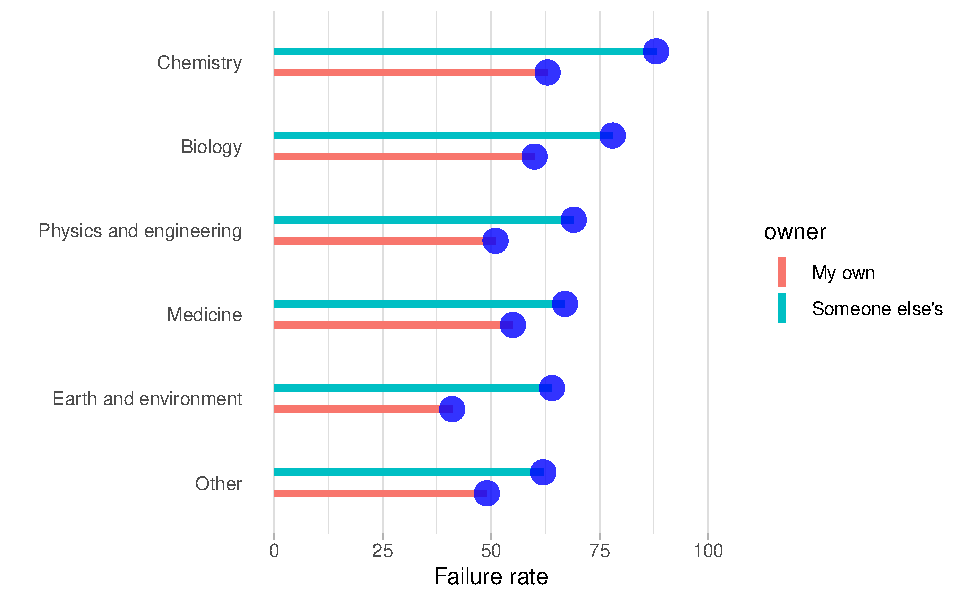
\includegraphics[width=0.9\textwidth]{figura32.pdf}
\caption{Reproducibility problems in different branches of science (data from \cite{baker20161})}
\label{figura32}
\end{figure}

\section{Characteristics of omic data}
\label{sec:charomicdata}
The word "omics" makes reference to the study of some characteristics of different families of biological molecules, such as genes, proteins, etc. The basic aspect of the omic approaches is that a complex system can be understood more thoroughly if considered as a whole. Thanks to this approach, the advances that have been achieved in the last decades in the understanding of the different biological processes are huge, and today the future of medicine and biology cannot be understood outside the view of the different omics approaches \parencite{van2018role}. In few years, omics technologies have given as an unimaginable deep knowledge of many celular proceses and pathways, helping the scientific community to make huge progresses in the understanding of living systems. Each year new technologies are developed allowing for the gathering of more information, increasing the resolution of the analyses and improving the precision of the determinations. As emerging fields, the different omics are still expanding and defining themselves but, in a general view, omic data can be classified according to the nature of the elements being analyzed. Following this approach, 5 different fields can be delimited (\autoref{figura01}):

\begin{itemize}
    \item Genomics: Focused at the structure, function, evolution and mapping of genomes, that is, the complete set of DNA of an organism.
    \item Epigenomics: Studies the complete set of epigenetic reversible modifications of the genome, which regulate expression.
    \item Transcriptomics: Focused at the whole set of RNA transcripts of an organism, that is, the expression of an organism's genes.
    \item Proteomics: Focused at the whole set of proteins produced or modified by an organism. Proteomics studies protein composition, structure and activity,
    \item Metabolomics: Studies metabolites in a biological entity, which are the end products of cellular processes
\end{itemize}

\begin{figure}[htbp]\centering
		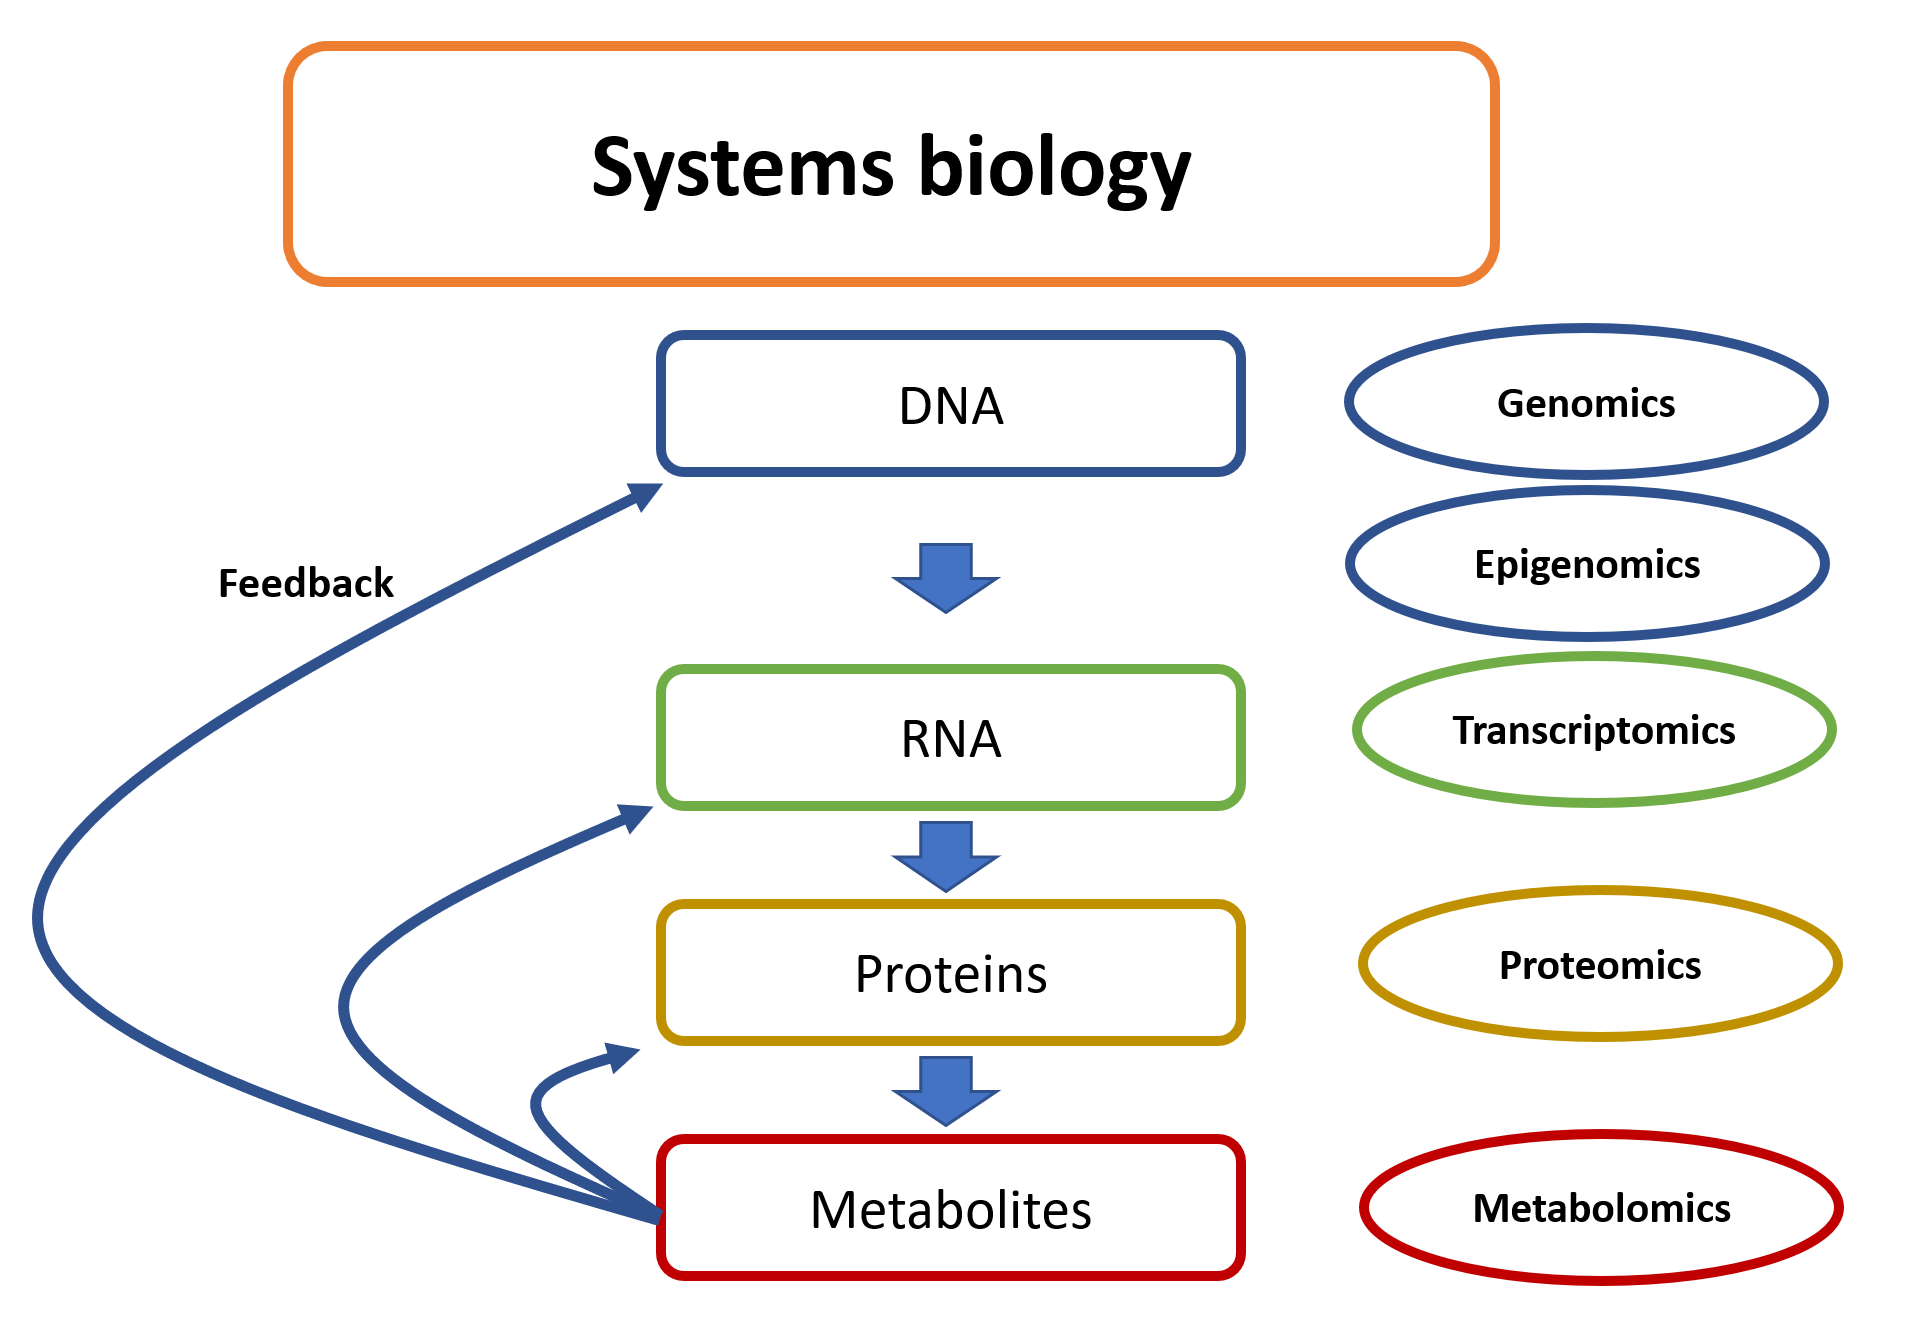
\includegraphics[width=.7\textwidth]{figura01}
		\caption{Different omic technologies and their relationship}
		\label{figura01}
	\end{figure}

For expanded information about the different omic fields, it is recommended the work of \cite{2018iv} and also the paper of \cite{horgan2011omic}.

\subsection{Metabolomic data}
The term '\textit{metabolome}' is used to address the entire set of metabolites present in an organism and '\textit{metabolomics}' is defined as the comprehensive and quantitative analysis of all metabolites of the biological system under study \parencite{fiehn2001combining}. Metabolomics studies the final products of the "omics downstream" presented in \autoref{figura01}, so its information is influenced by the actions of genomic, epigenomic, transcriptomic and proteomic mechanisms. Because of this, metabolomics is the closest approximation to phenotype among all omic technologies, thus providing  more information about the actual status of the organism than the others \parencite{beger2016metabolomics}. 

In general metabolomic studies can be classified as targeted or untargeted depending on whether the researcher measures and quantifies a specific set of known metabolites or the largest possible number of metabolites contained in a biological system. 
Among all omic technologies, metabolomics is the most complex and heterogeneous. More specifically, targeted metabolomic studies focus on accurate identification and quantification of a defined set of metabolites in biological samples which was predetermined by the scientific question formulated by the researcher or, in some cases, by the size of metabolite library that is available in the software used for the analyses. On the other hand, untargeted metabolomics focuses on measuring and comparing as many signals as possible in a biological samples, and then assigning these signals to specific metabolites by using annotation databases. It is important to mention that a significant portion of the detected signals cannot be identified because their are missing in the annotation databases. A typical raw data spectrum of a metabolomics analysis is presented in \autoref{figura37}.

\begin{figure}[htbp]\centering
		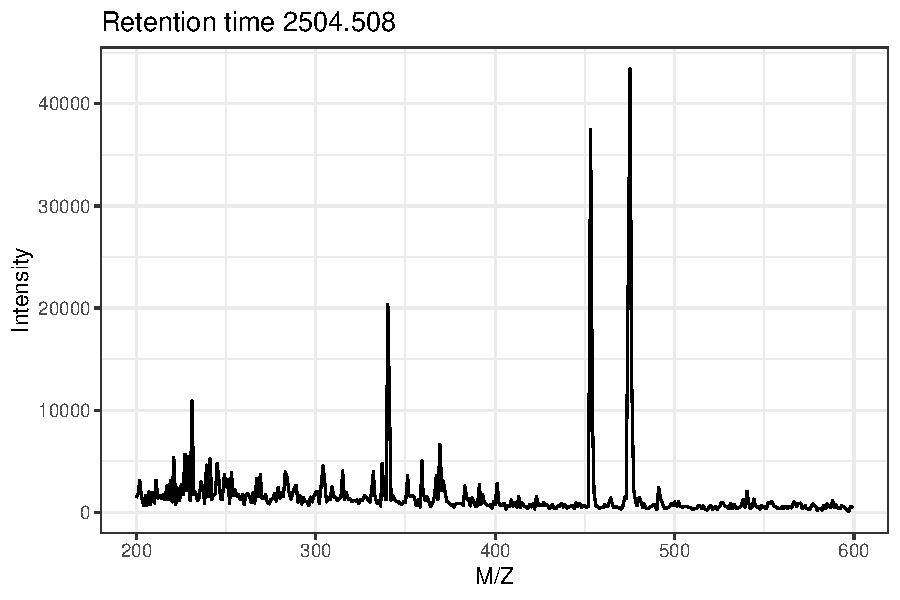
\includegraphics[width=.7\textwidth]{figura37.pdf}
		\caption{Raw spectrum of a metabolomics analysis}
		\label{figura37}
	\end{figure}

In genomics, epigenomics and transcriptomics, measurement procedures are reasonably standardized. This is not the case in metabolomics, with many different technologies being used, which lead to different study designs and different produced data types \parencite{moco2007metabolomics}. The commonly used analytical techniques for metabolomic studies are nuclear magnetic resonance (NMR), spectroscopy and mass spectrometry \parencite{buscher2009cross}. Another specific hurdle of metabolomics is the identification of the metabolites in untargeted analyses. Many of the metabolites found in an untargeted analysis can not be identified, because the data bases for associating a specific mass and retention time to a concrete metabolite are still very immature \parencite{mathew2013metabolomics}. In fact, identification of unknowns is considered as the bottleneck of untargeted metabolomics \parencite{bingol2018recent}.
In any case, although heterogeneous, metabolomic data share a common set of properties which define their most important characteristics for their statistical analysis:

\begin{itemize}
    \item High correlation among variables
    \item Complex pre-processing of the signal to obtain the data
    \item High range of detection values among variables
    \item Variables (metabolites) found in one analysis are not guaranteed to be found in a subsequent analysis
\end{itemize}

All these properties add to the difficulty of analyzing metabolomic data, as will be further developed in the next section.

\section{Challenges for analyzing metabolomic data}
\label{sec:challengesmetabodata}
Traditionally, omic data analyses have been performed using classical statistical methods from last century. In most cases, these methods consisted in bivariate tests such as \textit{t test} or \textit{Wilcoxon-Mann Whitney test}, followed by some sort of multiple comparissons correction such as \textit{Bonferroni} or \textit{False Discovery Rate} \parencite{hochberg1990more, benjamini1995controlling}. These approaches suffer from several drawbacks including lack of statistical power, lack of interpretability of results, and omission of complex relationships among variables. Thus, classical statistical methods based on bivariate tests are not adequate to extract all the information available in omic data sets.
Some of the mentioned problems such as the lack of interpretability or the omission of complex relationships could be adressed using statistical models such as linear models or generalized liner models, but these methods also suffer from other problems when dealing with omic data, such as the large number of variables and low sample size, which produces overfitting, and the high correlation among variables, which produces multicollinearity. All these obstacles for omic data analysis have motivated the development of numerous novel statistical techniques during the last decades specifically aimed at solving them. Methods such as PLS \parencite{wold1984collinearity}, lasso \parencite{tibshirani1996regression}, elastic net \parencite{zou2005regularization} and random forest \parencite{breiman2001random}, among others, can deal with most of the problems exposed in the preceding lines. Nevertheless, other challenges remain partially unresolved, such as the analysis of repeated measures data or, more generally, data organized in multiway arrays. Also, in a discipline where the number of variables is so large, the development of variable selection methods is of utmost importance.

\section{Strategies and aims of the thesis}
\label{sec:strategiesthesis}
As presented in the previous sections, omic data sets and, more specifically, metabolomic data sets contain a large amount of information in the form of huge data structures. The magnitude of this data sets dificults their handling and also their analysis and interpretation. Additionally, metabolomics presents specific singularities that make necessary the use of complex pre-processing and analysis techniques. The aim of metabolomic analyses is the identification of those metabolites related to the specific biological question being studied. As of today, the majority of statistical analyses performed on metabolomic data sets are based on classical methods or, in the best cases, on adequate but limited modern statistical methods. Among these adequate methods stand out principal component analysis (PCA), partial least squares (PLS), penalization methods such as ridge or lasso and other machine learning techniques such as random forest or boosting. However, these techniques are not able no deal effectively with all the particularities of metabolomic data sets. Their limitations get clearly exposed when dealing with data sets with repeated measurements over time or, more generally, three-way or multi-way data sets. An important part of the work on this thesis will consist on critically reviewing an assessing the usefulness of the different presented tools for metabolomic data analysis. 
Some useful tool for analyzing three-way data are the Tucker3 and PARAFAC models and, when some \textbf{Y} data structure is to be predicted, the $N$-PLS model. Related to the problem of these datasets with a large number of features, comes the issue of variable selection. Variable selection is essential for facilitating e.g. biological interpretation of the results when analyzing “-omic” data sets. It is often the case that the aim of these analyses is to find a new biomarker or a specific set of biomarkers, also called signature, to diagnose or predict the prognosis of a disease. For this cases, the $N$-PLS algorithm does not provide variable selection implemented within the algorithm, although some methods have been developed to perform it after the fitting of the model. One of the main research lines of this thesis will be the introduction of L1-penalization in the $N$-PLS algorithm to allow for variable selection at the model-fitting step. This approach should not only facilitate interpretation by producing a reduced model including fewer variables, but should also reduce prediction error by completely eliminating noise features instead of downweghting them as $N$-PLS does. 
The full list of objectives for this thesis is presented below:

\begin{itemize}
    \item Try, assess and evaluate different preprocessing techniques for metabolomic data
    \item Study and critically evaluate the use of different modern data analysis techniques for dealing with metabolomic data sets.
    \item Develop a novel algorithm based on the combination of $N$-PLS and L1-penalization for the analysis of three- or multi-way datasets that allows for variable selection at the model-fitting step
    \item Develop a software package based in the R language, that implements the new algorithm along with all the extra functions needed for performing complete analyses of three-way data sets and their posterior interpretation.
\end{itemize}
